\begin{figure}[p]
    \centering
    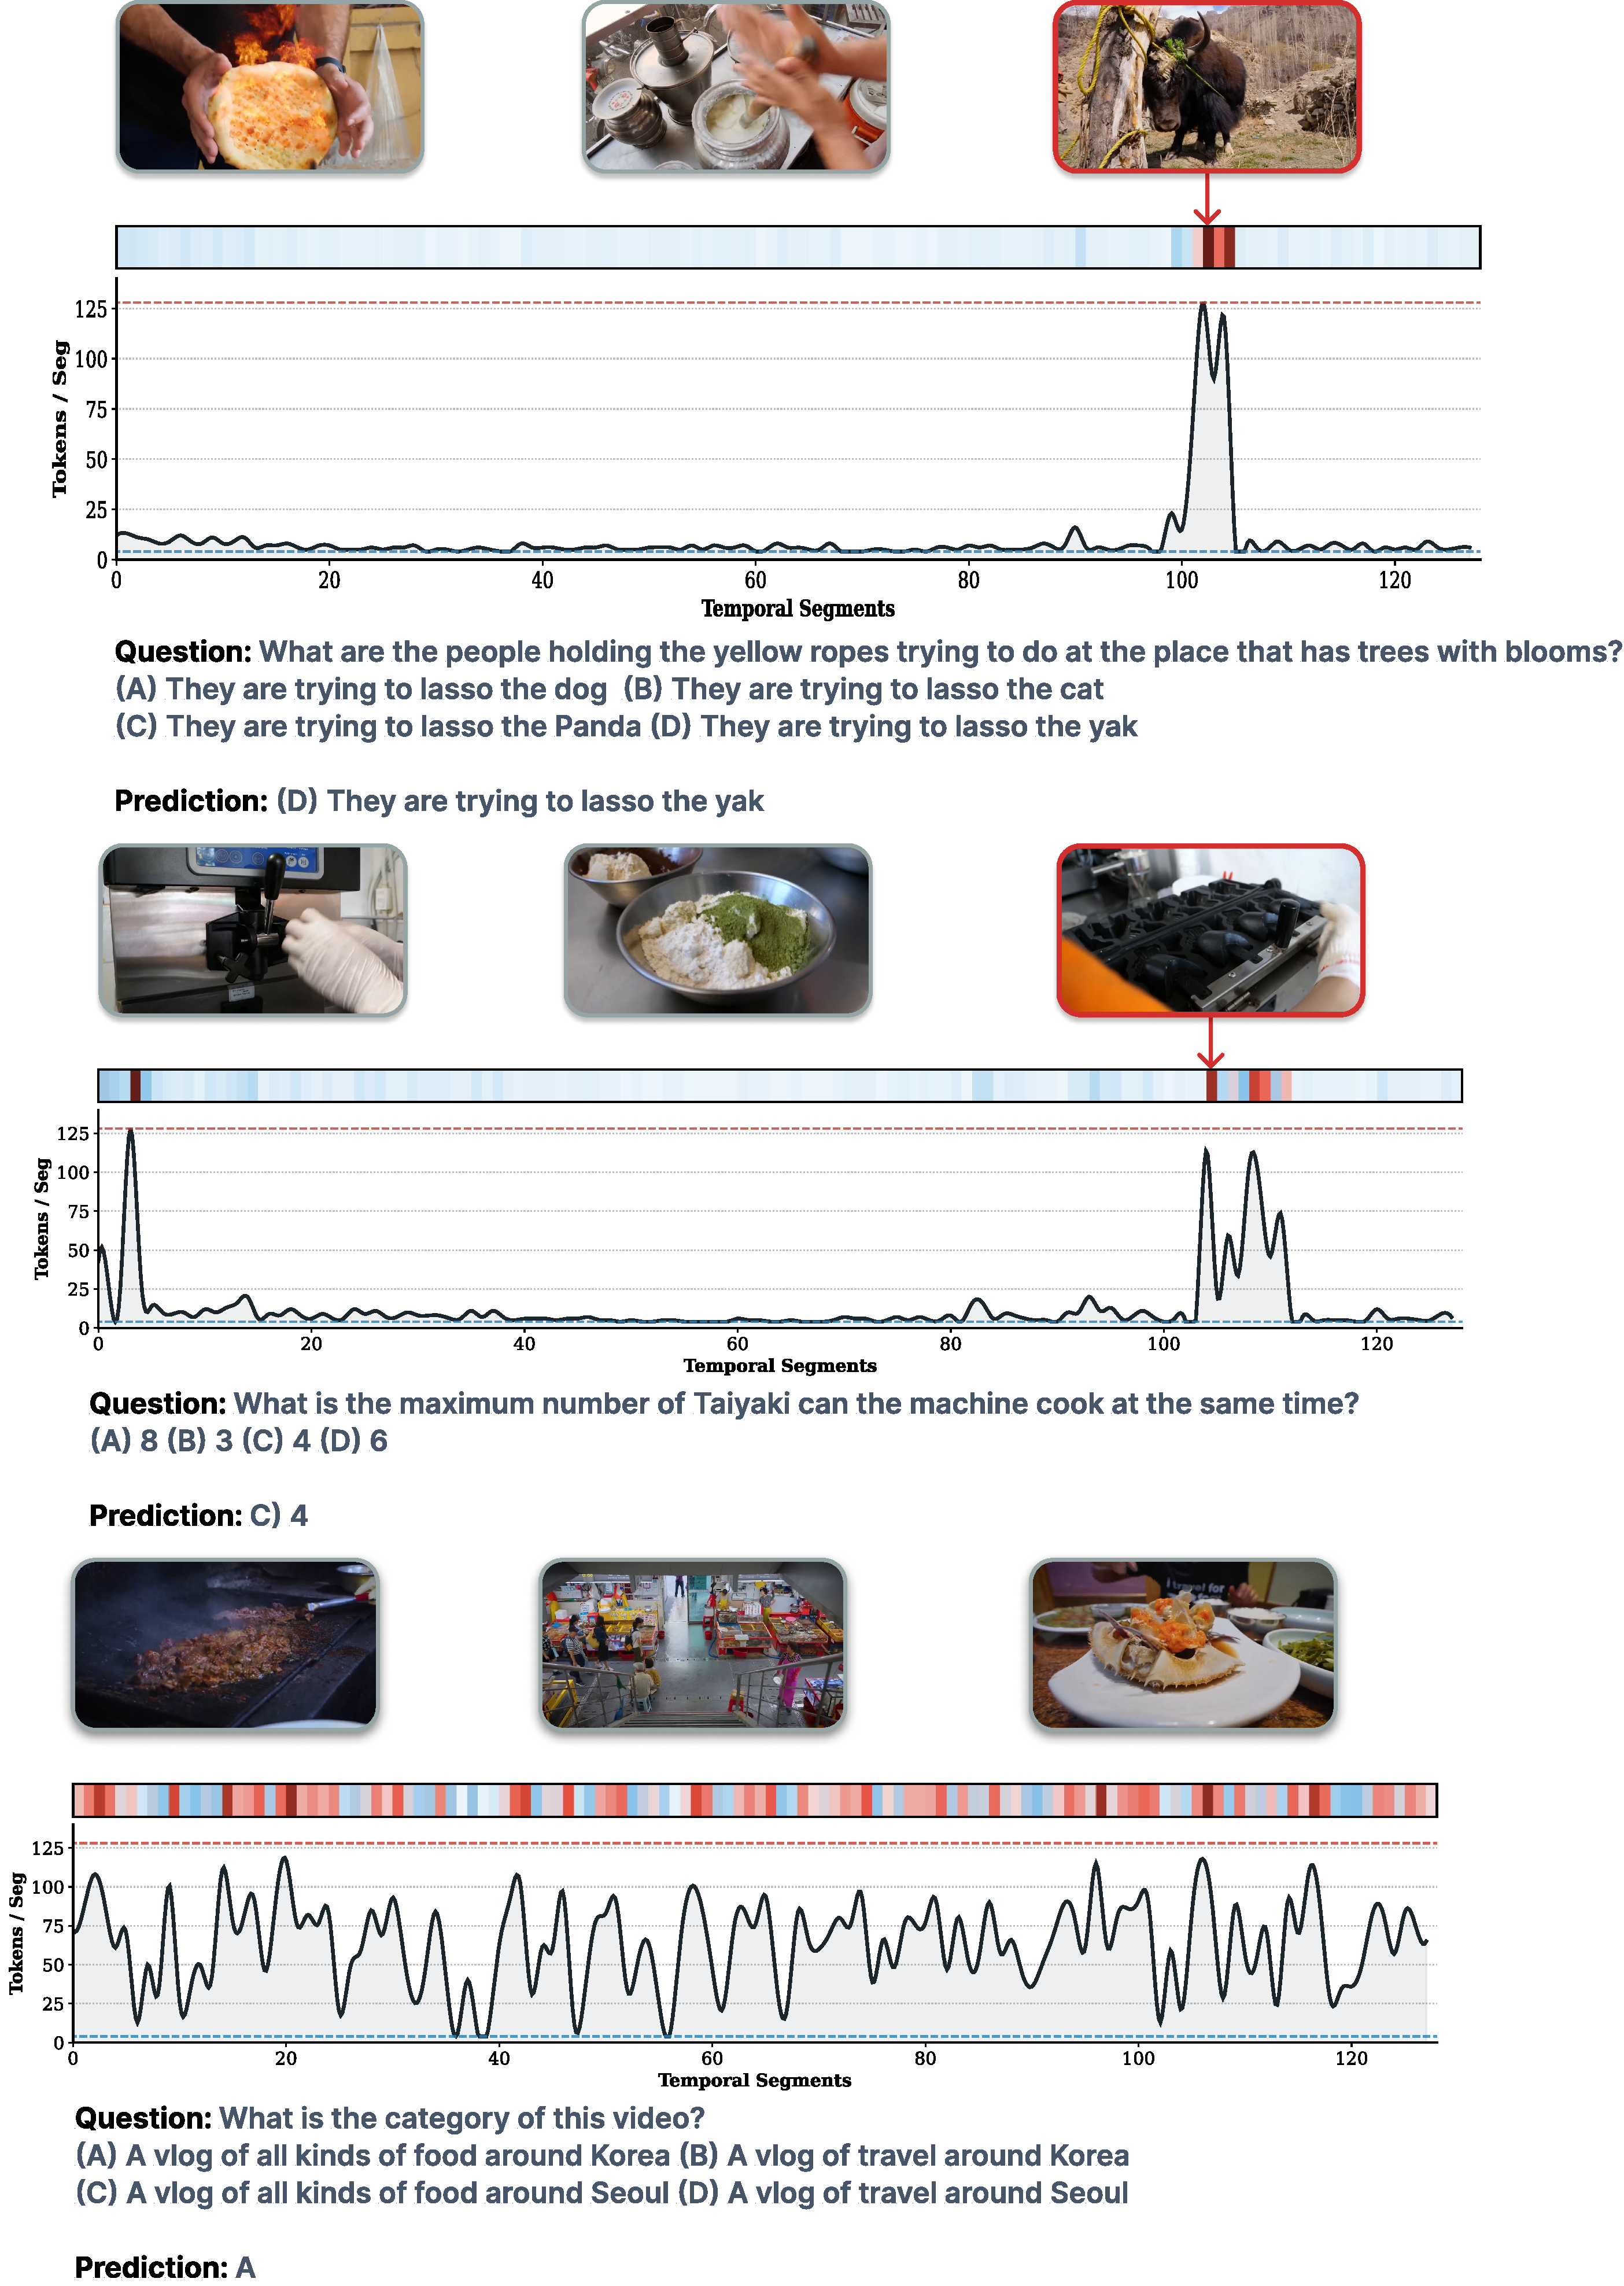
\includegraphics[width=0.88\textwidth]{supp/fig/demo.pdf}
    % \caption{
    % \textbf{Qualitative examples of query-aware Adaptive Token Allocation.} We visualize the token allocation distribution across three distinct types of video QA. The red-bordered key frames correspond to segments with high token allocation, while grey-bordered frames represent redundant contexts compressed to minimal tokens. 
    % \textbf{(Top) Precise Retrieval:} ATA isolates the exact moment the text appears. 
    % \textbf{(Middle) Event Localization:} ATA highlights the specific scenes (the boat) relevant to the query while suppressing irrelevant scenes. 
    % \textbf{(Bottom) Global Summarization:} ATA maintains a dense allocation distribution to capture the overall theme of the video.
    % }
    \caption{
        \textbf{Qualitative examples of query-aware Adaptive Token Allocation.} We visualize the token allocation distribution across three distinct types of video QA. The red-bordered key frames correspond to segments with high token allocation, while grey-bordered frames represent redundant contexts compressed to minimal tokens. 
        \textbf{(Top) Precise Action Retrieval:} ATA isolates the exact moment the target action (lassoing the yak) occurs. 
        \textbf{(Middle) Targeted Object Grounding:} ATA highlights specific scenes containing cooking machinery relevant to the query concepts (``machine'', ``cook''), while effectively suppressing general manual food preparation. 
        \textbf{(Bottom) Global Summarization:} ATA maintains a dense allocation distribution to capture the overarching theme of the diverse food vlog.
    }
    \label{fig:qual_demo}
\end{figure}